\documentclass[11pt,a4paper]{article}

% ============================================
% PACKAGES - Language & Encoding
% ============================================
\usepackage[T5]{fontenc}  % T5 encoding for Vietnamese
\usepackage[utf8]{inputenc}  % UTF-8 input encoding
\usepackage[vietnamese]{babel}  % Vietnamese language support
\usepackage{indentfirst}

% ============================================
% PACKAGES - Math & Symbols
% ============================================
\usepackage{amsmath}
\usepackage{amsfonts}
\usepackage{amssymb}

% ============================================
% PACKAGES - Graphics & Figures
% ============================================
\usepackage{graphicx}  % graphicx includes all graphics functionality
\usepackage{tikz}
\usetikzlibrary{patterns,calc,angles}  % Combined TikZ libraries
\usepackage{float}

% ============================================
% PACKAGES - Tables & Layout
% ============================================
\usepackage{array}
\usepackage{multirow}
\usepackage{booktabs}
\usepackage{caption}
\usepackage{subcaption}

% ============================================
% PACKAGES - Page Layout
% ============================================
\usepackage[left=2cm, right=2cm, top=2cm, bottom=2cm]{geometry}
\usepackage{setspace}
\onehalfspacing
\usepackage{fancyhdr}
\usepackage[bottom]{footmisc}

% ============================================
% PACKAGES - Lists & Enumerations
% ============================================
\usepackage{enumitem}
\setlist{nolistsep}

% ============================================
% PACKAGES - Code Listings
% ============================================
\usepackage{listings}
\usepackage{xcolor}

% Define colors for code
\definecolor{codegreen}{rgb}{0,0.6,0}
\definecolor{codegray}{rgb}{0.5,0.5,0.5}
\definecolor{codepurple}{rgb}{0.58,0,0.82}
\definecolor{backcolour}{rgb}{0.95,0.95,0.92}

% PHP Style
\lstdefinestyle{phpstyle}{
    language=PHP,
    backgroundcolor=\color{backcolour},   
    commentstyle=\color{codegreen},
    keywordstyle=\color{blue}\bfseries,
    numberstyle=\tiny\color{codegray},
    stringstyle=\color{codepurple},
    basicstyle=\ttfamily\footnotesize,
    breakatwhitespace=false,         
    breaklines=true,                 
    captionpos=b,                    
    keepspaces=true,                 
    numbers=left,                    
    numbersep=5pt,                  
    showspaces=false,                
    showstringspaces=false,
    showtabs=false,                  
    tabsize=4
}

% HTML Style
\lstdefinestyle{htmlstyle}{
    language=HTML,
    backgroundcolor=\color{backcolour},   
    commentstyle=\color{codegreen},
    keywordstyle=\color{blue}\bfseries,
    numberstyle=\tiny\color{codegray},
    stringstyle=\color{codepurple},
    basicstyle=\ttfamily\footnotesize,
    breaklines=true,
    captionpos=b,
    numbers=left,
    tabsize=2
}

% CSS Style
\lstdefinestyle{cssstyle}{
    language=CSS,
    backgroundcolor=\color{backcolour},   
    commentstyle=\color{codegreen},
    keywordstyle=\color{magenta}\bfseries,
    numberstyle=\tiny\color{codegray},
    stringstyle=\color{codepurple},
    basicstyle=\ttfamily\footnotesize,
    breaklines=true,
    captionpos=b,
    numbers=left,
    tabsize=2
}

% JavaScript Style
\lstdefinestyle{jsstyle}{
    language=Java,
    backgroundcolor=\color{backcolour},   
    commentstyle=\color{codegreen},
    keywordstyle=\color{blue}\bfseries,
    numberstyle=\tiny\color{codegray},
    stringstyle=\color{codepurple},
    basicstyle=\ttfamily\footnotesize,
    breaklines=true,
    captionpos=b,
    numbers=left,
    tabsize=2
}

\lstset{style=phpstyle} % Default style

% ============================================
% PACKAGES - Hyperlinks & References
% ============================================
\usepackage{hyperref}
\hypersetup{
    colorlinks=true,
    linkcolor=blue,
    filecolor=magenta,      
    urlcolor=cyan,
    citecolor=blue,
    pdftitle={Báo cáo BTL Lập trình Web},
    pdfauthor={Nhóm L01\_6},
}

% ============================================
% PACKAGES - Others
% ============================================
\usepackage{mdframed}
\usepackage{mathptmx}
\usepackage{titlesec}


% ============================================
% FORMATTING - Section Titles
% ============================================
\titleformat{\section}{\fontsize{13.5}{15}\selectfont\bfseries}{\thesection}{1em}{}
\titleformat{\subsection}{\fontsize{13.25}{15}\selectfont\bfseries}{\thesubsection}{1em}{}
\titleformat{\subsubsection}{\fontsize{13}{15}\selectfont\bfseries}{\thesubsubsection}{1em}{}

% ============================================
% FORMATTING - Headers & Footers
% ============================================
\pagestyle{fancy}
\fancyhf{}
\lhead{\textit{BÀI TẬP LỚN LẬP TRÌNH WEB}}
\rhead{\textit{Nhóm L01\_6}}
\rfoot{Trang \thepage}
\lfoot{\textit{GVHD: Nguyễn Hữu Hiếu}}
\renewcommand{\footrulewidth}{0.4pt}
\renewcommand{\headrulewidth}{0.4pt}
\setlength{\headheight}{14.97527pt}

% ============================================
% CUSTOM COMMANDS & ENVIRONMENTS
% ============================================
\newmdenv[linewidth=0.6pt,linecolor=black,skipabove=\topsep,skipbelow=\topsep,
leftmargin=-5pt,rightmargin=-5pt,
innerleftmargin=5pt,innerrightmargin=5pt]{mybox}

\newcommand\tab[1][0.7cm]{\hspace*{#1}}
\setlength{\skip\footins}{0.5cm}

% ============================================
% DOCUMENT START
% ============================================
\begin{document}

% Roman page numbering for front matter
\pagenumbering{roman}

% ============================================
% TITLE PAGE
% ============================================
\begin{titlepage}
    \begin{center}
    \LARGE \textbf{ĐẠI HỌC QUỐC GIA THÀNH PHỐ HỒ CHÍ MINH} \\
    \vspace{0.2cm}
    \LARGE \textbf{TRƯỜNG ĐẠI HỌC BÁCH KHOA} \\
    \vspace{0.2cm}
    \LARGE \textbf{KHOA KHOA HỌC VÀ KĨ THUẬT MÁY TÍNH}
    \end{center}
    
    \vspace{0.3cm}
    
    \begin{figure}[h!]
    \begin{center}
    \includegraphics[width=4cm]{Images/hcmut.png}
    \end{center}
    \end{figure}

    \begin{center}
    \begin{tabular}{c}
    \multicolumn{1}{c}{\textbf{{\LARGE BÁO CÁO BÀI TẬP LỚN}}}\\
    \\{\textbf{{\LARGE LẬP TRÌNH WEB (HK1 2025-2026)}}}
    \\
    \\
    \textbf{\LARGE Thiết kế giao diện và xây dựng các tính năng cơ bản }\\
    \textbf{\LARGE  cho website công ty - doanh nghiệp}
    \end{tabular}
    \vspace{1.5cm}

    \end{center}
    \hspace{3.5cm} {\Large \textbf{GIẢNG VIÊN HƯỚNG DẪN:} Nguyễn Hữu Hiếu} \vspace{0.5cm}
    \par
    \hspace{3cm} {\Large \textbf{Lớp:} L01} \vspace {0.5cm} 
    \par
    \hspace{3cm} {\Large \textbf{DANH SÁCH THÀNH VIÊN:}} 
    \vspace{0.5cm}
    \begin{center}
        \begin{tabular}{|c|c|c|}
        \hline
        \textbf{STT}  &\textbf{Họ và tên} & \textbf{MSSV}\\
        \hline
            1 & Hoàng Hữu Hà & 2113271\\ 
        \hline
            2 & Lê Bảo Linh & 2311849\\ 
        \hline
            3 & Nguyễn Trung Hiếu & 2113357\\
        \hline
            4 & Hà Thế Bình & 2152435\\
        \hline
        \end{tabular}
    \end{center}
    \vspace{2cm}
    \begin{center}
        {\Large Thành phố Hồ Chí Minh - 12/2025 }
    \end{center}
\end{titlepage}
\newpage

% ============================================
% TABLE OF CONTENTS
% ============================================
\tableofcontents
\newpage

\listoffigures
\newpage

\listoftables
\newpage

% Arabic page numbering for main content
\pagenumbering{arabic}

% ============================================
% MAIN CONTENT
% ============================================

% ============================================
% CHƯƠNG 1: GIỚI THIỆU
% ============================================

\section{Giới thiệu}

% ------------------------------------------
\subsection{Website thương mại điện tử}

Trong thời đại công nghệ số ngày nay, thương mại điện tử (E-commerce) đã trở thành một phần không thể thiếu trong đời sống kinh tế - xã hội. Website thương mại điện tử là nền tảng cho phép doanh nghiệp và người tiêu dùng thực hiện các giao dịch mua bán trực tuyến một cách thuận tiện và nhanh chóng.

Các đặc điểm nổi bật của website thương mại điện tử:
\begin{itemize}
    \item \textbf{Tiếp cận rộng:} Không giới hạn về địa lý, khách hàng có thể truy cập mọi lúc mọi nơi
    \item \textbf{Chi phí thấp:} Giảm chi phí vận hành so với cửa hàng truyền thống
    \item \textbf{Cá nhân hóa:} Đề xuất sản phẩm phù hợp với từng khách hàng
    \item \textbf{Dữ liệu phân tích:} Thu thập và phân tích hành vi người dùng
\end{itemize}

Theo xu hướng phát triển, các website thương mại điện tử ngày càng chú trọng đến trải nghiệm người dùng (UX), tốc độ tải trang, và tính bảo mật trong giao dịch.

% ------------------------------------------
\subsection{Template Fahasa}

Fahasa.com là một trong những website bán sách trực tuyến hàng đầu tại Việt Nam, thuộc công ty cổ phần Phát hành Sách TP.HCM (FAHASA). Website cung cấp đa dạng các loại sách từ sách giáo khoa, văn học, self-help đến các sản phẩm văn phòng phẩm và đồ chơi.

\textbf{Đặc điểm nổi bật của Fahasa:}
\begin{itemize}
    \item Giao diện thân thiện, dễ sử dụng
    \item Hệ thống phân loại sách rõ ràng theo thể loại
    \item Tính năng tìm kiếm mạnh mẽ
    \item Giỏ hàng và thanh toán trực tuyến tiện lợi
    \item Chương trình khuyến mãi và tích điểm cho thành viên
\end{itemize}

Dự án này lấy cảm hứng từ giao diện và các tính năng của Fahasa.com để xây dựng một website thương mại điện tử bán sách hoàn chỉnh.

% ------------------------------------------
\subsection{Mục tiêu của dự án}

\textbf{Mục tiêu học tập:}
\begin{enumerate}
    \item Hiểu và áp dụng kiến trúc MVC (Model-View-Controller) trong PHP
    \item Nắm vững các công nghệ frontend: HTML5, CSS3, JavaScript, Bootstrap
    \item Thực hành xây dựng ứng dụng web full-stack
    \item Hiểu về quy trình phát triển phần mềm theo nhóm
\end{enumerate}

\textbf{Sản phẩm cuối cùng:}
\begin{itemize}
    \item Website thương mại điện tử bán sách hoàn chỉnh
    \item Tài liệu báo cáo chi tiết về dự án
    \item Source code có cấu trúc rõ ràng, dễ bảo trì
\end{itemize}

% ------------------------------------------
\subsection{Phạm vi báo cáo}

\textbf{Các tính năng đã xây dựng:}
\begin{itemize}
    \item Trang chủ với banner và sản phẩm nổi bật
    \item Danh sách sản phẩm với tìm kiếm và lọc
    \item Chi tiết sản phẩm
    \item Giỏ hàng (thêm, xóa, cập nhật số lượng)
    \item Trang thông tin khách hàng (profile, đơn hàng, wishlist)
    \item Trang tin tức và chi tiết bài viết
    \item Trang giới thiệu, hỏi đáp và liên hệ
    \item Đăng nhập/Đăng ký (Frontend mockup)
\end{itemize}

\textbf{Công nghệ sử dụng:}
\begin{itemize}
    \item \textbf{Frontend:} HTML5, CSS3, Bootstrap 5, JavaScript
    \item \textbf{Backend:} PHP 7.0+ với mô hình MVC tự xây dựng
    \item \textbf{Icons:} Font Awesome 6
    \item \textbf{Server:} XAMPP (Apache)
\end{itemize}

\textbf{Giới hạn của dự án:}
\begin{itemize}
    \item Sử dụng dữ liệu mock thay vì database thực
    \item Chưa tích hợp thanh toán trực tuyến
    \item Chưa có panel quản trị hoàn chỉnh
\end{itemize}

\newpage

% ============================================
% CHƯƠNG 2: CƠ SỞ LÝ THUYẾT
% ============================================

\section{Cơ sở lý thuyết}

% ------------------------------------------
\subsection{Công nghệ Frontend}

\subsubsection{HTML5}

HTML5 (HyperText Markup Language version 5) là phiên bản mới nhất của ngôn ngữ đánh dấu siêu văn bản, được sử dụng để cấu trúc và trình bày nội dung trên web.

\textbf{Các tính năng mới của HTML5:}
\begin{itemize}
    \item \textbf{Semantic Elements:} Các thẻ có ý nghĩa như \texttt{<header>}, \texttt{<nav>}, \texttt{<section>}, \texttt{<article>}, \texttt{<footer>} giúp cấu trúc trang web rõ ràng hơn
    \item \textbf{Form Elements:} Các input types mới như \texttt{email}, \texttt{date}, \texttt{tel}, \texttt{number} với validation tự động
    \item \textbf{Multimedia:} Hỗ trợ \texttt{<video>} và \texttt{<audio>} native
    \item \textbf{Canvas \& SVG:} Vẽ đồ họa trực tiếp trên trình duyệt
\end{itemize}

\subsubsection{CSS3}

CSS3 (Cascading Style Sheets Level 3) là phiên bản mới nhất của CSS, cung cấp các tính năng styling mạnh mẽ cho web.

\textbf{Các tính năng quan trọng:}
\begin{itemize}
    \item \textbf{Flexbox:} Layout một chiều linh hoạt cho việc căn chỉnh và phân bố không gian
    \item \textbf{CSS Grid:} Layout hai chiều mạnh mẽ cho các thiết kế phức tạp
    \item \textbf{Transitions \& Animations:} Tạo hiệu ứng chuyển động mượt mà
    \item \textbf{Media Queries:} Responsive design cho nhiều kích thước màn hình
    \item \textbf{Custom Properties:} CSS Variables cho quản lý styles dễ dàng
\end{itemize}

\subsubsection{Bootstrap 5}

Bootstrap là framework CSS phổ biến nhất, giúp xây dựng giao diện responsive nhanh chóng.

\textbf{Ưu điểm của Bootstrap 5:}
\begin{itemize}
    \item Hệ thống Grid 12 cột linh hoạt
    \item Các components có sẵn: Navbar, Cards, Modals, Forms
    \item Không phụ thuộc jQuery (khác với phiên bản cũ)
    \item Utility classes phong phú
    \item Documentation chi tiết và cộng đồng lớn
\end{itemize}

\textbf{Nhược điểm:}
\begin{itemize}
    \item Kích thước file CSS lớn nếu không tối ưu
    \item Giao diện dễ bị "Bootstrap look" nếu không customize
\end{itemize}

\subsubsection{JavaScript}

JavaScript là ngôn ngữ lập trình phía client, giúp tạo tương tác động trên trang web.

\textbf{Các tính năng ES6+ sử dụng trong dự án:}
\begin{itemize}
    \item \texttt{let/const}: Khai báo biến có phạm vi block
    \item \texttt{Arrow functions}: Cú pháp hàm ngắn gọn
    \item \texttt{Template literals}: String interpolation với backticks
    \item \texttt{DOM manipulation}: querySelector, addEventListener
    \item \texttt{Fetch API}: Gọi API bất đồng bộ
    \item \texttt{LocalStorage}: Lưu trữ dữ liệu trên trình duyệt
\end{itemize}

% ------------------------------------------
\subsection{Công nghệ Backend}

\subsubsection{PHP}

PHP (Hypertext Preprocessor) là ngôn ngữ lập trình phía server phổ biến, đặc biệt trong phát triển web.

\textbf{Đặc điểm của PHP:}
\begin{itemize}
    \item Dễ học và triển khai
    \item Tích hợp tốt với HTML
    \item Hỗ trợ nhiều database (MySQL, PostgreSQL, SQLite)
    \item Cộng đồng lớn và nhiều framework (Laravel, Symfony)
\end{itemize}

\textbf{Các tính năng PHP sử dụng:}
\begin{itemize}
    \item Sessions để quản lý trạng thái người dùng
    \item Autoloading với \texttt{spl\_autoload\_register}
    \item Object-oriented programming
    \item URL routing với \texttt{.htaccess}
\end{itemize}

\subsubsection{Mô hình MVC}

MVC (Model-View-Controller) là kiến trúc phần mềm phân tách ứng dụng thành 3 thành phần:

\begin{itemize}
    \item \textbf{Model:} Xử lý logic nghiệp vụ và tương tác với dữ liệu
    \item \textbf{View:} Hiển thị giao diện người dùng
    \item \textbf{Controller:} Nhận request, xử lý logic và trả về response
\end{itemize}

\textbf{Lợi ích của MVC:}
\begin{enumerate}
    \item Tách biệt rõ ràng giữa logic và giao diện
    \item Dễ bảo trì và mở rộng
    \item Hỗ trợ làm việc nhóm hiệu quả
    \item Tái sử dụng code cao
\end{enumerate}

% ------------------------------------------
\subsection{Bảo mật ứng dụng web}

\subsubsection{Session Security}

Session là cơ chế lưu trữ thông tin người dùng trên server giữa các request.

\textbf{Các biện pháp bảo mật session:}
\begin{itemize}
    \item Regenerate session ID sau khi đăng nhập
    \item Đặt timeout cho session
    \item Sử dụng HTTPS để mã hóa session cookie
    \item Kiểm tra User-Agent và IP address
\end{itemize}

\subsubsection{XSS Prevention}

Cross-Site Scripting (XSS) là lỗ hổng cho phép attacker chèn mã JavaScript độc hại.

\textbf{Phòng chống XSS:}
\begin{itemize}
    \item Sử dụng \texttt{htmlspecialchars()} khi output dữ liệu
    \item Content Security Policy (CSP) headers
    \item Validate và sanitize input
\end{itemize}

\subsubsection{SQL Injection Prevention}

SQL Injection xảy ra khi attacker chèn mã SQL vào input để thao túng database.

\textbf{Phòng chống:}
\begin{itemize}
    \item Sử dụng Prepared Statements với PDO
    \item Validate input type và length
    \item Giới hạn quyền database user
\end{itemize}

\subsubsection{CSRF Protection}

Cross-Site Request Forgery lừa người dùng thực hiện hành động không mong muốn.

\textbf{Phòng chống CSRF:}
\begin{itemize}
    \item Sử dụng CSRF tokens trong forms
    \item Kiểm tra Origin/Referer headers
    \item SameSite cookie attribute
\end{itemize}

% ------------------------------------------
\subsection{SEO cơ bản}

Search Engine Optimization giúp website được tìm thấy dễ dàng trên các công cụ tìm kiếm.

\textbf{Các yếu tố SEO on-page:}
\begin{itemize}
    \item \textbf{Title tags:} Tiêu đề trang ngắn gọn, có keyword
    \item \textbf{Meta description:} Mô tả hấp dẫn dưới 160 ký tự
    \item \textbf{Heading hierarchy:} Sử dụng H1-H6 đúng cách
    \item \textbf{Semantic HTML:} Giúp search engine hiểu cấu trúc trang
    \item \textbf{URL thân thiện:} URLs ngắn, có ý nghĩa
    \item \textbf{Image alt text:} Mô tả hình ảnh cho accessibility và SEO
    \item \textbf{Page speed:} Tốc độ tải trang ảnh hưởng ranking
\end{itemize}

\newpage

% ============================================
% CHƯƠNG 3: THIẾT KẾ ỨNG DỤNG
% ============================================

\section{Thiết kế ứng dụng}

% ------------------------------------------
\subsection{Thiết kế cơ sở dữ liệu}

Mặc dù dự án hiện tại sử dụng dữ liệu mock, thiết kế database được xây dựng với tầm nhìn mở rộng trong tương lai.

\textbf{Sơ đồ các entities chính:}

\begin{table}[H]
\centering
\begin{tabular}{|l|l|l|}
\hline
\textbf{Tên trường} & \textbf{Kiểu dữ liệu} & \textbf{Mô tả} \\
\hline
id & INT (PK) & Khóa chính, auto increment \\
username & VARCHAR(50) & Tên đăng nhập \\
email & VARCHAR(100) & Email người dùng \\
password & VARCHAR(255) & Mật khẩu đã hash \\
fullname & VARCHAR(100) & Họ tên đầy đủ \\
phone & VARCHAR(15) & Số điện thoại \\
address & TEXT & Địa chỉ giao hàng \\
role & ENUM & 'customer', 'admin' \\
created\_at & DATETIME & Thời gian tạo tài khoản \\
\hline
\end{tabular}
\caption{Bảng Users - Quản lý người dùng}
\label{tab:users}
\end{table}

\begin{table}[H]
\centering
\begin{tabular}{|l|l|l|}
\hline
\textbf{Tên trường} & \textbf{Kiểu dữ liệu} & \textbf{Mô tả} \\
\hline
id & INT (PK) & Khóa chính \\
name & VARCHAR(200) & Tên sản phẩm \\
slug & VARCHAR(200) & URL-friendly name \\
description & TEXT & Mô tả chi tiết \\
price & DECIMAL(10,2) & Giá bán \\
original\_price & DECIMAL(10,2) & Giá gốc \\
image & VARCHAR(255) & Đường dẫn hình ảnh \\
category\_id & INT (FK) & Liên kết bảng categories \\
author & VARCHAR(100) & Tác giả sách \\
stock & INT & Số lượng tồn kho \\
\hline
\end{tabular}
\caption{Bảng Products - Quản lý sản phẩm}
\label{tab:products}
\end{table}

\begin{table}[H]
\centering
\begin{tabular}{|l|l|l|}
\hline
\textbf{Tên trường} & \textbf{Kiểu dữ liệu} & \textbf{Mô tả} \\
\hline
id & INT (PK) & Khóa chính \\
user\_id & INT (FK) & Liên kết bảng users \\
total & DECIMAL(12,2) & Tổng tiền đơn hàng \\
status & ENUM & 'processing', 'shipping', 'completed', 'cancelled' \\
shipping\_address & TEXT & Địa chỉ giao hàng \\
created\_at & DATETIME & Thời gian đặt hàng \\
\hline
\end{tabular}
\caption{Bảng Orders - Quản lý đơn hàng}
\label{tab:orders}
\end{table}

% ------------------------------------------
\subsection{Kiến trúc MVC tự xây dựng}

Dự án áp dụng mô hình MVC (Model-View-Controller) được xây dựng hoàn toàn từ đầu, không sử dụng framework có sẵn như Laravel hay Symfony. Điều này giúp hiểu sâu về cách thức hoạt động của pattern MVC.

\subsubsection{Luồng hoạt động MVC}

\begin{figure}[H]
\centering
\begin{tikzpicture}[node distance=2cm, auto,
    box/.style={rectangle, draw, fill=blue!20, text width=3cm, text centered, rounded corners, minimum height=1cm},
    arrow/.style={->,>=stealth,thick}]

    \node[box] (user) {User Request};
    \node[box, below of=user] (router) {Router (App.php)};
    \node[box, below of=router] (controller) {Controller};
    \node[box, left of=controller, node distance=6cm] (model) {Model};
    \node[box, right of=controller, node distance=6cm] (view) {View};
    \node[box, below of=controller] (response) {HTTP Response};

    \draw[arrow] (user) -- (router);
    \draw[arrow] (router) -- node[right] {Parse URL} (controller);
    \draw[arrow] (controller) -- node[above] {Query} (model);
    \draw[arrow] (model) -- node[below] {Data} (controller);
    \draw[arrow] (controller) -- node[above] {Render} (view);
    \draw[arrow] (view) -- node[below] {HTML} (controller);
    \draw[arrow] (controller) -- (response);
\end{tikzpicture}
\caption{Luồng xử lý request trong mô hình MVC}
\label{fig:mvc-flow}
\end{figure}

\subsubsection{Các thành phần Core}

\textbf{1. Router - App.php:}
\begin{itemize}
    \item Parse URL thành: \texttt{[controller, method, params]}
    \item Load controller tương ứng
    \item Gọi method với parameters
    \item Xử lý 404 nếu không tìm thấy
\end{itemize}

\textbf{2. Base Controller - Controller.php:}
\begin{itemize}
    \item \texttt{model(\$name)}: Load model động
    \item \texttt{view(\$view, \$data)}: Render view với data
    \item \texttt{redirect(\$path)}: Chuyển hướng trang
    \item \texttt{isPost()}, \texttt{isGet()}: Kiểm tra HTTP method
\end{itemize}

\textbf{3. Database Wrapper - DB.php:}
\begin{itemize}
    \item PDO connection singleton
    \item \texttt{query(\$sql, \$params)}: Execute với prepared statements
    \item \texttt{single()}, \texttt{all()}: Fetch results
    \item Transaction support
\end{itemize}


% ------------------------------------------
\subsection{Cấu trúc thư mục}

Dự án được tổ chức theo cấu trúc MVC rõ ràng:

\begin{verbatim}
BTL_Fahasa/
|-- app/                      # Application code
|   |-- config/               # Configuration files
|   |-- controllers/          # Controller classes
|   |-- core/                 # Core framework files
|   |-- models/               # Model classes
|   +-- views/                # View templates
|-- public/                   # Public assets
|   |-- index.php             # Entry point
|   |-- css/                  # Stylesheets
|   |-- js/                   # JavaScript files
|   +-- images/               # Images
+-- db/                       # Database files
\end{verbatim}


% ------------------------------------------
\subsection{Tính năng hệ thống}

\subsubsection{Khách (Guest)}

Người dùng chưa đăng nhập có thể:
\begin{itemize}
    \item Truy cập trang chủ và xem sản phẩm nổi bật
    \item Duyệt danh sách sản phẩm theo danh mục
    \item Xem chi tiết sản phẩm
    \item Tìm kiếm sản phẩm
    \item Đọc tin tức và bài viết
    \item Xem trang giới thiệu, hỏi đáp, liên hệ
    \item Đăng ký tài khoản mới
    \item Đăng nhập vào hệ thống
\end{itemize}

\subsubsection{Thành viên (Customer)}

Sau khi đăng nhập, thành viên có thêm các quyền:
\begin{itemize}
    \item Thêm sản phẩm vào giỏ hàng
    \item Quản lý giỏ hàng (tăng/giảm số lượng, xóa)
    \item Xem và chỉnh sửa thông tin cá nhân
    \item Xem lịch sử đơn hàng
    \item Quản lý danh sách sản phẩm yêu thích
    \item Nhận thông báo về đơn hàng
    \item Đăng xuất khỏi hệ thống
\end{itemize}

\subsubsection{Quản trị viên (Admin)}

\textit{Lưu ý: Tính năng admin chưa được triển khai đầy đủ trong phiên bản hiện tại.}

Các tính năng dự kiến:
\begin{itemize}
    \item Quản lý danh sách người dùng
    \item Thêm/sửa/xóa sản phẩm
    \item Quản lý danh mục sản phẩm
    \item Xử lý đơn hàng
    \item Quản lý nội dung tin tức
    \item Xem thống kê và báo cáo
\end{itemize}

% ------------------------------------------
\subsection{Luồng hoạt động (Flowcharts)}

\textbf{Luồng đăng nhập:}
\begin{enumerate}
    \item Người dùng truy cập trang đăng nhập
    \item Nhập username và password
    \item Hệ thống kiểm tra thông tin
    \item Nếu đúng: Tạo session, redirect về trang chủ
    \item Nếu sai: Hiển thị thông báo lỗi
\end{enumerate}

\textbf{Luồng mua hàng:}
\begin{enumerate}
    \item Khách hàng duyệt sản phẩm
    \item Click "Thêm vào giỏ" trên sản phẩm mong muốn
    \item Kiểm tra đăng nhập - nếu chưa, yêu cầu đăng nhập
    \item Sản phẩm được thêm vào giỏ hàng (Session)
    \item Khách hàng có thể tiếp tục mua hoặc checkout
    \item Xem giỏ hàng, điều chỉnh số lượng
    \item Tiến hành thanh toán
    \item Xác nhận đơn hàng
\end{enumerate}

\newpage

% ============================================
% CHƯƠNG 4: HIỆN THỰC
% ============================================

\section{Hiện thực}

Chương này trình bày chi tiết các trang và tính năng đã xây dựng trong dự án, kèm theo hình ảnh minh họa.

% ------------------------------------------
\subsection{Giao diện trang chủ}

Trang chủ là điểm tiếp xúc đầu tiên với người dùng, được thiết kế với bố cục rõ ràng và hấp dẫn.

\textbf{Các thành phần chính:}
\begin{itemize}
    \item \textbf{Header:} Logo, thanh tìm kiếm, navigation menu, icon giỏ hàng và tài khoản
    \item \textbf{Banner:} Slider quảng cáo sản phẩm nổi bật
    \item \textbf{Featured Products:} Grid hiển thị sản phẩm được đề xuất
    \item \textbf{Categories:} Danh mục sách theo thể loại
    \item \textbf{Footer:} Thông tin liên hệ, links, social media
\end{itemize}

\begin{figure}[H]
\centering
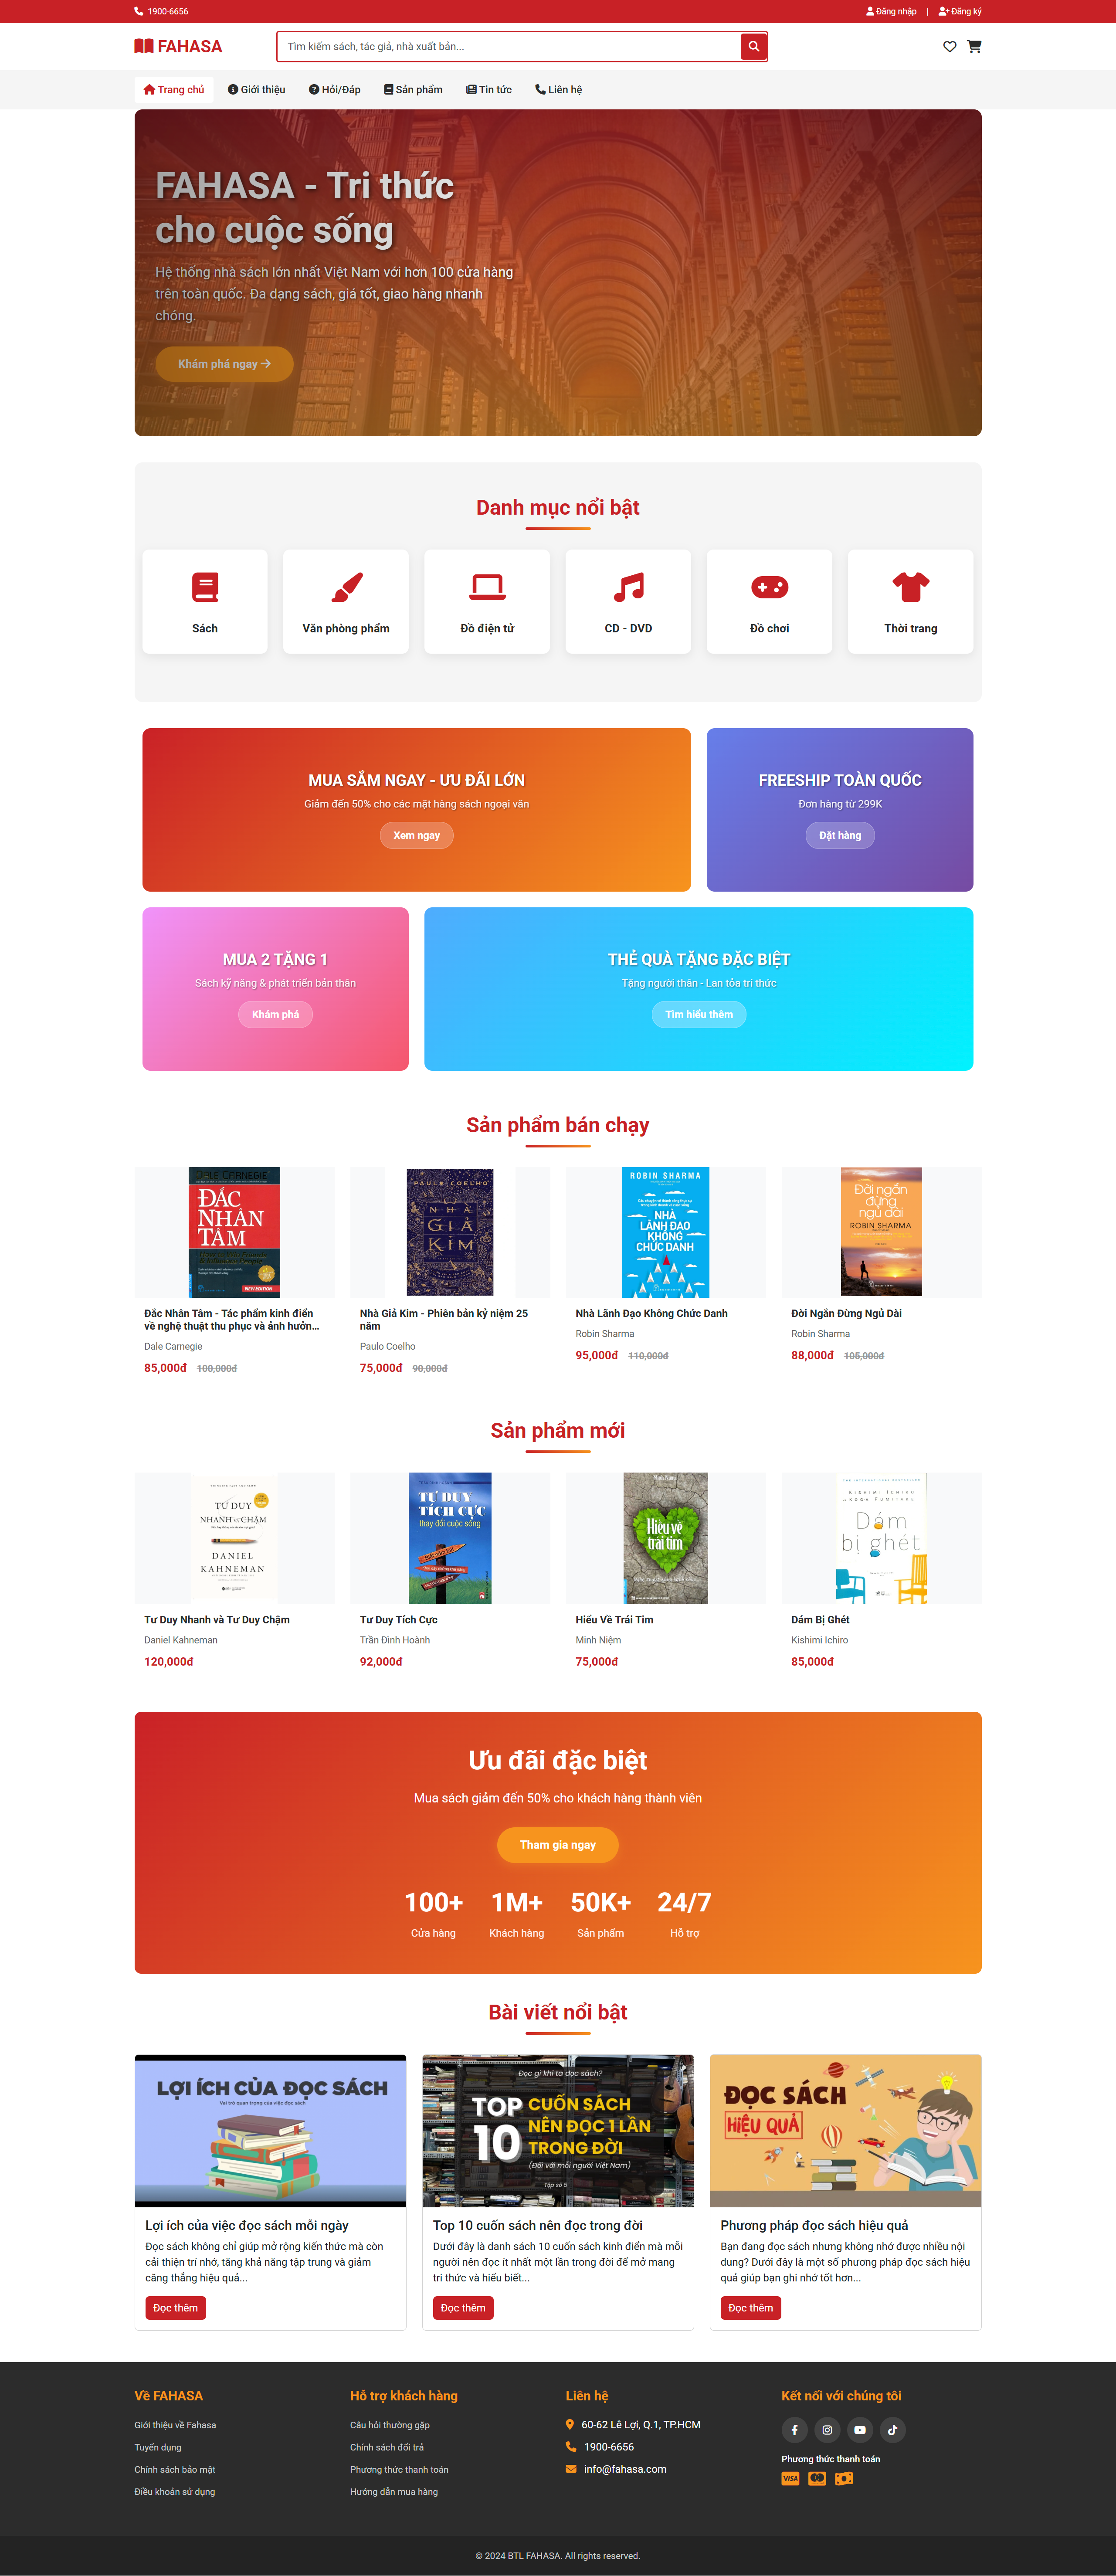
\includegraphics[width=0.6\textwidth]{Images/home_page.png}
\caption{Giao diện trang chủ Fahasa Clone}
\label{fig:home}
\end{figure}

% ------------------------------------------
\subsection{Trang sản phẩm}

\subsubsection{Danh sách sản phẩm}

Trang danh sách hiển thị tất cả sản phẩm với các tính năng:
\begin{itemize}
    \item Grid layout responsive (4 cột desktop, 2 cột mobile)
    \item Card sản phẩm với hình ảnh, tên, giá, badge giảm giá
    \item Lọc theo danh mục
    \item Sắp xếp theo giá, tên, newest
    \item Pagination
\end{itemize}

\begin{figure}[H]
\centering
\includegraphics[width=0.6\textwidth]{Images/product_list.png}
\caption{Trang danh sách sản phẩm}
\label{fig:product-list}
\end{figure}

\subsubsection{Chi tiết sản phẩm}

Trang chi tiết cung cấp thông tin đầy đủ về một sản phẩm:
\begin{itemize}
    \item Hình ảnh sản phẩm lớn, có thể zoom
    \item Thông tin: tên, tác giả, giá gốc, giá khuyến mãi
    \item Mô tả chi tiết sản phẩm
    \item Nút "Thêm vào giỏ" và "Mua ngay"
    \item Sản phẩm liên quan
\end{itemize}

\begin{figure}[H]
\centering
\includegraphics[width=0.6\textwidth]{Images/product_detail.png}
\caption{Trang chi tiết sản phẩm}
\label{fig:product-detail}
\end{figure}

% ------------------------------------------
\subsection{Giỏ hàng}

Tính năng giỏ hàng cho phép người dùng quản lý các sản phẩm đã chọn mua.

\textbf{Các chức năng:}
\begin{itemize}
    \item Xem danh sách sản phẩm trong giỏ
    \item Tăng/giảm số lượng với nút +/-
    \item Xóa sản phẩm khỏi giỏ
    \item Tính toán tự động tổng tiền
    \item Hiển thị số lượng sản phẩm trên icon giỏ hàng
\end{itemize}

\begin{figure}[H]
\centering
\includegraphics[width=0.7\textwidth]{Images/cart_page.png}
\caption{Trang giỏ hàng}
\label{fig:cart}
\end{figure}

\textbf{Xử lý phía server:}

CartController xử lý các action:
\begin{itemize}
    \item \texttt{index()}: Hiển thị giỏ hàng
    \item \texttt{add()}: Thêm sản phẩm
    \item \texttt{update()}: Cập nhật số lượng
    \item \texttt{remove()}: Xóa sản phẩm
\end{itemize}

Giỏ hàng được lưu trong \texttt{\$\_SESSION['cart']} dưới dạng array.

% ------------------------------------------
\subsection{Trang khách hàng}

\subsubsection{Thông tin tài khoản}

Cho phép người dùng xem và chỉnh sửa thông tin cá nhân:
\begin{itemize}
    \item Họ tên, email, số điện thoại
    \item Giới tính, ngày sinh
    \item Địa chỉ giao hàng
\end{itemize}

\begin{figure}[H]
\centering
\includegraphics[width=0.7\textwidth]{Images/customer_profile.png}
\caption{Trang thông tin tài khoản}
\label{fig:profile}
\end{figure}

\subsubsection{Đơn hàng của tôi}

Hiển thị lịch sử đơn hàng với các filter:
\begin{itemize}
    \item Tất cả đơn hàng
    \item Đang xử lý
    \item Đang giao
    \item Hoàn thành
    \item Đã hủy
\end{itemize}

\begin{figure}[H]
\centering
\includegraphics[width=0.7\textwidth]{Images/my_order.png}
\caption{Trang đơn hàng của tôi}
\label{fig:orders}
\end{figure}

\subsubsection{Thông báo}

Hiển thị các thông báo hệ thống về đơn hàng, khuyến mãi:

\begin{figure}[H]
\centering
\includegraphics[width=0.7\textwidth]{Images/notifications.png}
\caption{Trang thông báo}
\label{fig:notifications}
\end{figure}

\subsubsection{Sản phẩm yêu thích}

Danh sách các sản phẩm được đánh dấu yêu thích:

\begin{figure}[H]
\centering
\includegraphics[width=0.7\textwidth]{Images/wishlist.png}
\caption{Trang sản phẩm yêu thích}
\label{fig:wishlist}
\end{figure}

% ------------------------------------------
\subsection{Trang tin tức}

\subsubsection{Danh sách bài viết}

Hiển thị các bài viết, tin tức về sách:

\begin{figure}[H]
\centering
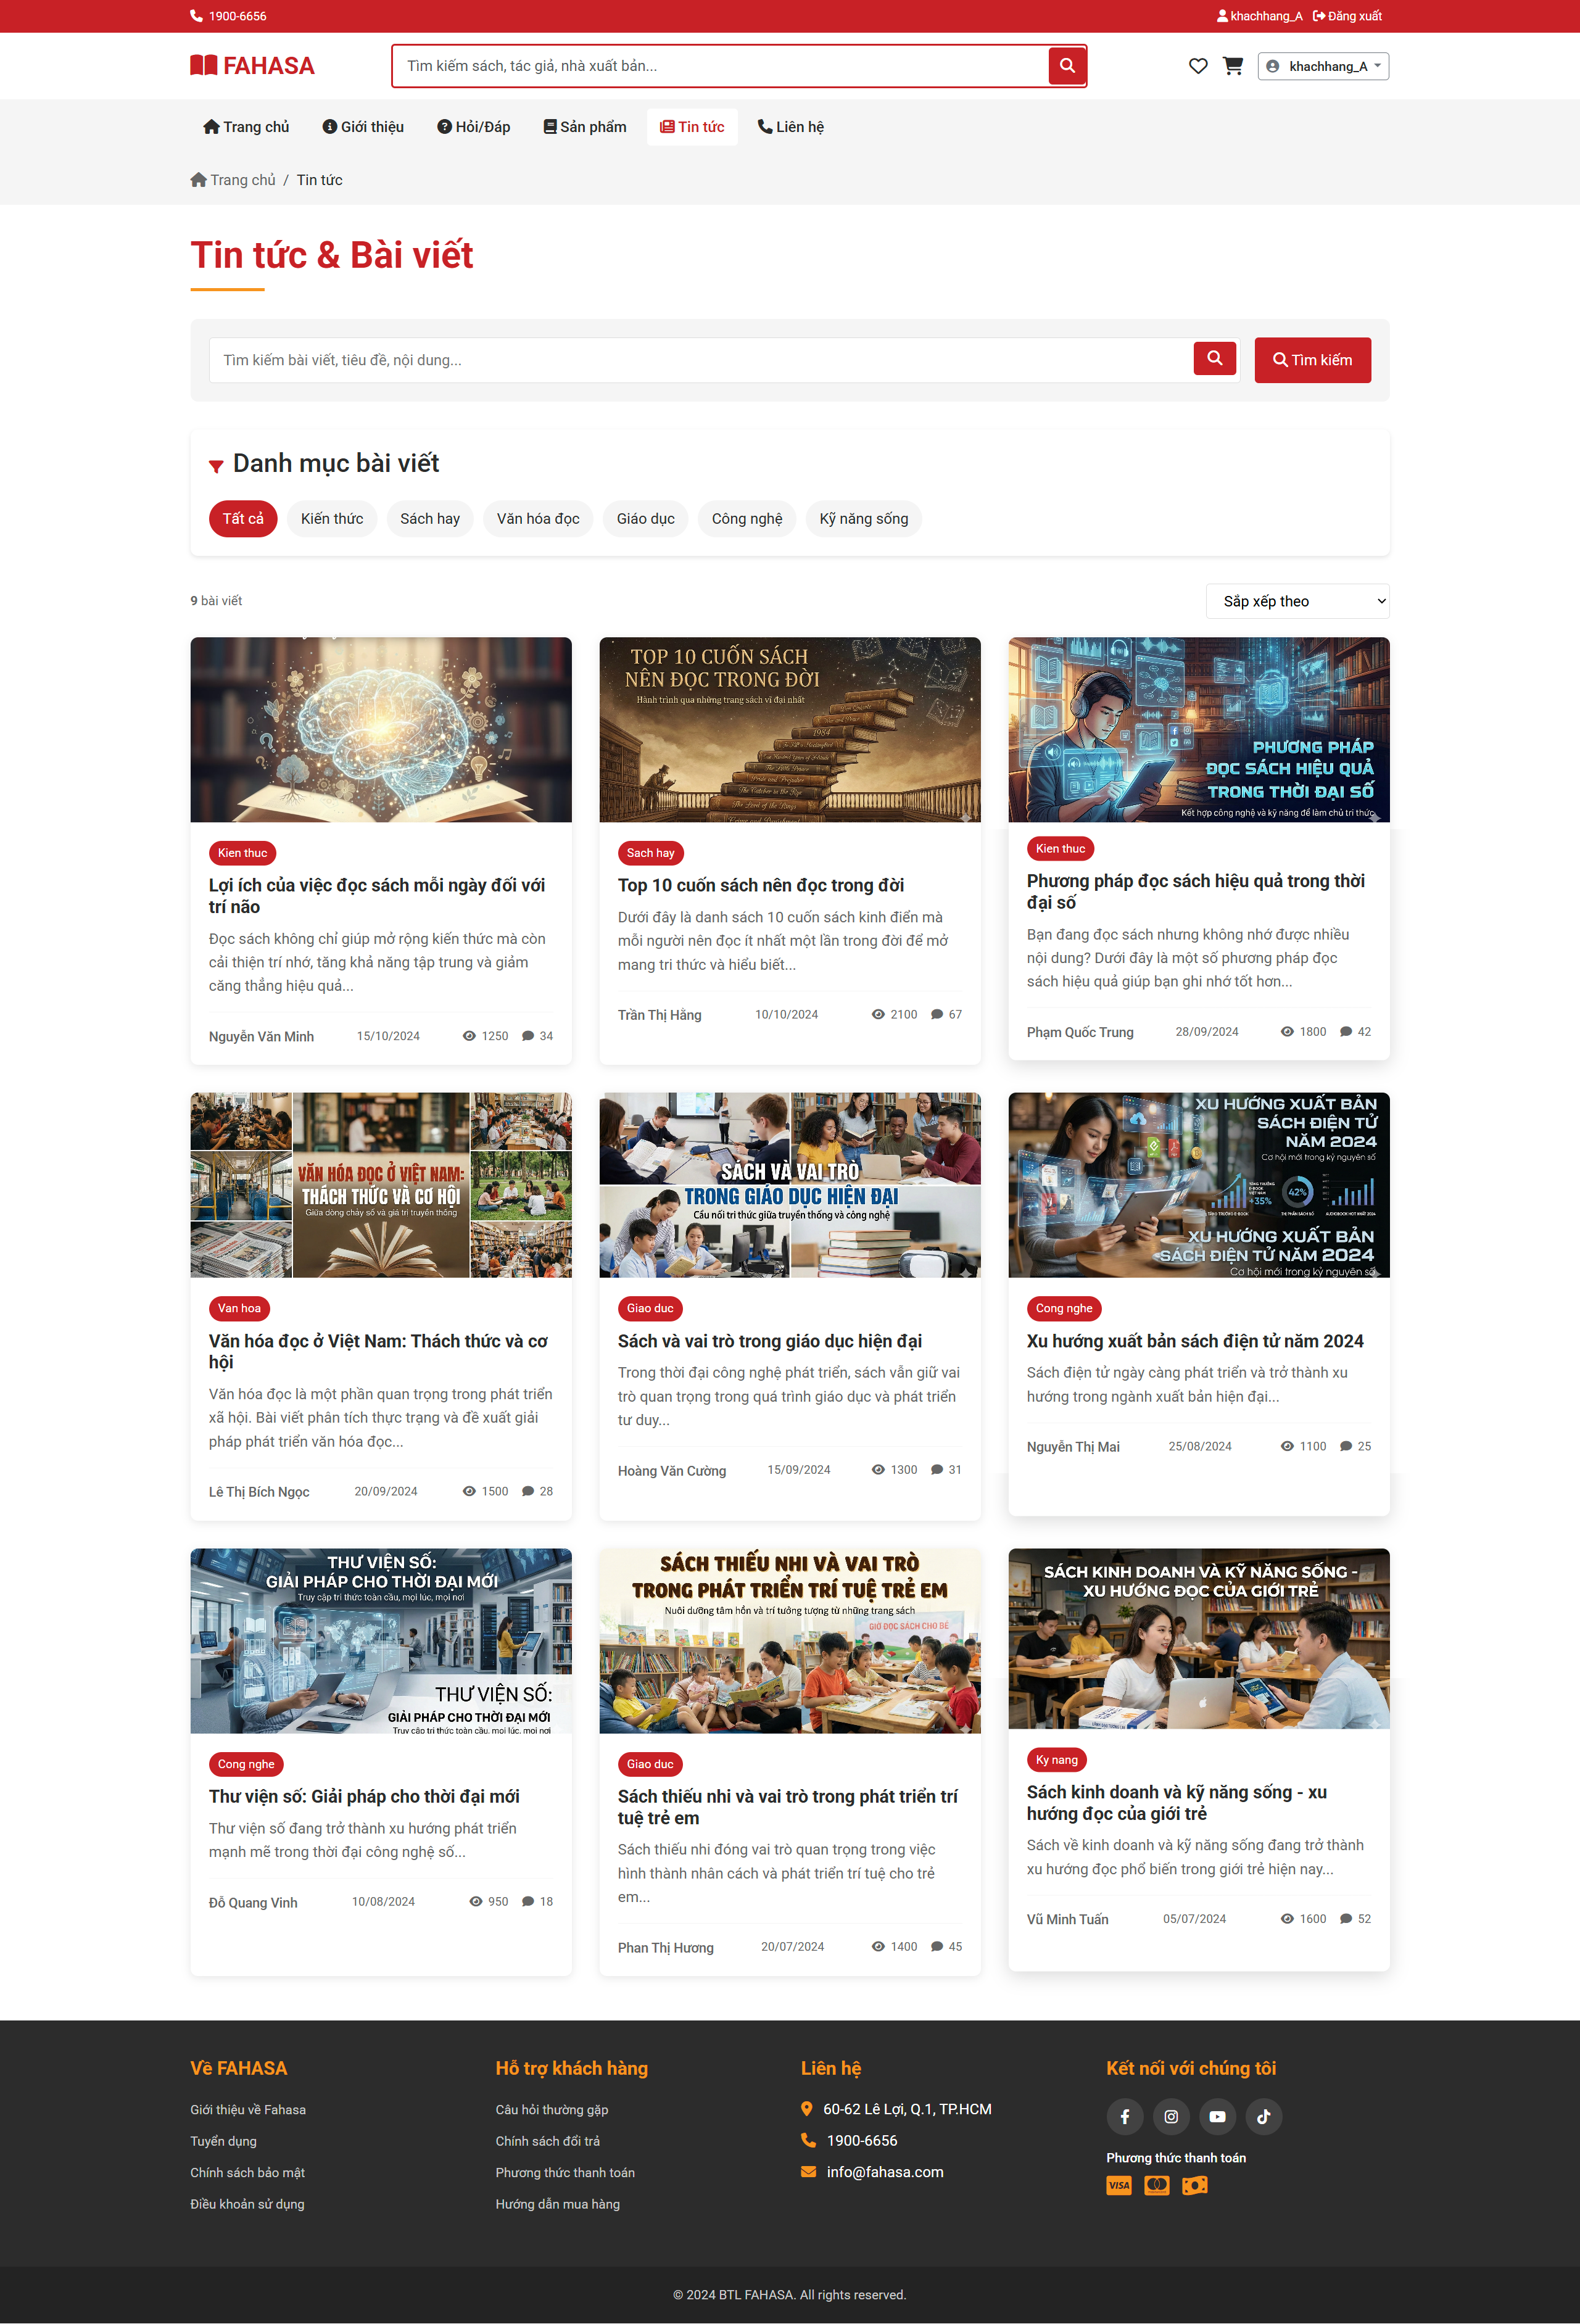
\includegraphics[width=0.6\textwidth]{Images/news_page.png}
\caption{Trang tin tức}
\label{fig:news}
\end{figure}

\subsubsection{Chi tiết bài viết}

Nội dung đầy đủ của bài viết, có phần bình luận:

\begin{figure}[H]
\centering
\includegraphics[width=0.6\textwidth]{Images/news_detail_page.png}
\caption{Trang chi tiết bài viết}
\label{fig:news-detail}
\end{figure}

% ------------------------------------------
\subsection{Các trang khác}

\subsubsection{Trang giới thiệu}

Giới thiệu về công ty Fahasa Clone:

\begin{figure}[H]
\centering
\includegraphics[width=0.6\textwidth]{Images/about_page.png}
\caption{Trang giới thiệu}
\label{fig:about}
\end{figure}

\subsubsection{Trang hỏi đáp}

FAQ - Câu hỏi thường gặp:

\begin{figure}[H]
\centering
\includegraphics[width=0.6\textwidth]{Images/qa_page.png}
\caption{Trang hỏi đáp}
\label{fig:qa}
\end{figure}

\subsubsection{Trang liên hệ}

Form liên hệ và thông tin công ty:

\begin{figure}[H]
\centering
\includegraphics[width=0.7\textwidth]{Images/contact_page.png}
\caption{Trang liên hệ}
\label{fig:contact}
\end{figure}

Giao diện Admin:

\begin{figure}[H]
\centering
\includegraphics[width=0.7\textwidth]{Images/dashboard_admin.jpg}
\caption{Trang Dashboard Admin}
\label{fig:dashboard_admin}
\end{figure}

\begin{figure}[H]
\centering
\includegraphics[width=0.7\textwidth]{Images/products_admin.jpg}
\caption{Trang Products Admin}
\label{fig:products_admin}
\end{figure}

\begin{figure}[H]
\centering
\includegraphics[width=0.7\textwidth]{Images/news_admin.jpg}
\caption{Trang Tin tức Admin}
\label{fig:news_admin}
\end{figure}

\begin{figure}[H]
\centering
\includegraphics[width=0.7\textwidth]{Images/contacts_admin.jpg}
\caption{Trang Contacts Admin}
\label{fig:contacts_admin}
\end{figure}

% ------------------------------------------
\subsection{Code snippets quan trọng}

\subsubsection{Router - App.php}

\begin{lstlisting}[style=phpstyle, caption=Core Router xử lý URL]
<?php
class App {
    protected $controller = 'HomeController';
    protected $method = 'index';
    protected $params = [];
    
    public function __construct() {
        $url = $this->parseUrl();
        
        // Load controller
        if(file_exists('../app/controllers/' . $url[0] . 'Controller.php')) {
            $this->controller = $url[0] . 'Controller';
            unset($url[0]);
        }
        
        require_once '../app/controllers/' . $this->controller . '.php';
        $this->controller = new $this->controller;
        
        // Call method
        if(isset($url[1]) && method_exists($this->controller, $url[1])) {
            $this->method = $url[1];
            unset($url[1]);
        }
        
        $this->params = $url ? array_values($url) : [];
        call_user_func_array([$this->controller, $this->method], $this->params);
    }
}
?>
\end{lstlisting}

\subsubsection{CartController - Thêm vào giỏ hàng}

\begin{lstlisting}[style=phpstyle, caption=Xử lý thêm sản phẩm vào giỏ]
<?php
public function add($productId = null) {
    if (!$productId) {
        $this->redirect('product');
    }
    
    // Get product info
    $product = $this->getProductById($productId);
    
    if ($product) {
        // Initialize cart if not exists
        if (!isset($_SESSION['cart'])) {
            $_SESSION['cart'] = [];
        }
        
        // Add or update quantity
        if (isset($_SESSION['cart'][$productId])) {
            $_SESSION['cart'][$productId]['quantity']++;
        } else {
            $_SESSION['cart'][$productId] = [
                'product' => $product,
                'quantity' => 1
            ];
        }
    }
    
    $this->redirect('cart');
}
?>
\end{lstlisting}

\subsubsection{JavaScript - Update Cart Quantity}

\begin{lstlisting}[style=jsstyle, caption=JavaScript xử lý tăng/giảm số lượng]
function updateQuantity(productId, action) {
    const input = document.querySelector(`#qty-${productId}`);
    let qty = parseInt(input.value);
    
    if (action === 'increase') {
        qty++;
    } else if (action === 'decrease' && qty > 1) {
        qty--;
    }
    
    input.value = qty;
    
    // Update via AJAX
    fetch(`/cart/update/${productId}/${qty}`, {
        method: 'POST'
    }).then(response => {
        updateCartTotal();
    });
}
\end{lstlisting}

\newpage

% ============================================
% CHƯƠNG 5: HƯỚNG DẪN CÀI ĐẶT
% ============================================

\section{Hướng dẫn cài đặt}

Chương này cung cấp hướng dẫn chi tiết để cài đặt và chạy dự án trên máy local.

% ------------------------------------------
\subsection{Yêu cầu hệ thống}

\textbf{Phần cứng tối thiểu:}
\begin{itemize}
    \item CPU: Intel Core i3 hoặc tương đương
    \item RAM: 4 GB
    \item Disk space: 500 MB trống
\end{itemize}

\textbf{Hệ điều hành:}
\begin{itemize}
    \item Windows 10/11
    \item macOS 10.15 trở lên
    \item Linux (Ubuntu 20.04+, Fedora, etc.)
\end{itemize}

\textbf{Phần mềm yêu cầu:}
\begin{itemize}
    \item XAMPP phiên bản 8.0 trở lên (bao gồm Apache và PHP)
    \item PHP phiên bản 7.4 trở lên (khuyến nghị 8.0+)
    \item Trình duyệt web hiện đại: Chrome, Firefox, Edge (phiên bản mới nhất)
    \item Git (tùy chọn, để clone project)
\end{itemize}

% ------------------------------------------
\subsection{Các bước cài đặt}

\subsubsection{Bước 1: Cài đặt XAMPP}

\begin{enumerate}
    \item Tải XAMPP từ \url{https://www.apachefriends.org/download.html}
    \item Chạy file installer
    \item Trong quá trình cài đặt, chọn các components:
    \begin{itemize}
        \item Apache (bắt buộc)
        \item PHP (bắt buộc)
        \item phpMyAdmin (tùy chọn, cho database)
    \end{itemize}
    \item Chọn thư mục cài đặt (mặc định: \texttt{C:\textbackslash xampp})
    \item Hoàn tất cài đặt
\end{enumerate}

\subsubsection{Bước 2: Clone hoặc copy project}

\textbf{Cách 1: Clone từ GitHub}
\begin{verbatim}
cd C:\xampp\htdocs
git clone https://github.com/Binh205/BTL_Fahasa.git
\end{verbatim}

\textbf{Cách 2: Copy thủ công}
\begin{enumerate}
    \item Giải nén file project
    \item Copy thư mục \texttt{BTL\_Fahasa} vào \texttt{C:\textbackslash xampp\textbackslash htdocs\textbackslash}
\end{enumerate}

\subsubsection{Bước 3: Khởi động Apache}

\begin{enumerate}
    \item Mở XAMPP Control Panel
    \item Click nút "Start" ở hàng Apache
    \item Đợi đến khi Apache chuyển sang màu xanh
    \item (Tùy chọn) Start MySQL nếu cần database
\end{enumerate}

\textbf{Lưu ý:} Nếu port 80 đã bị chiếm, có thể đổi sang port khác (ví dụ 8080):
\begin{enumerate}
    \item Click "Config" $\rightarrow$ "httpd.conf"
    \item Thay đổi \texttt{Listen 80} thành \texttt{Listen 8080}
    \item Thay đổi \texttt{ServerName localhost:80} thành \texttt{ServerName localhost:8080}
    \item Lưu file và restart Apache
\end{enumerate}

% ------------------------------------------
\subsection{Cấu hình}

\subsubsection{File config.php}

Mở file \texttt{app/config/config.php} và kiểm tra các settings:

\begin{lstlisting}[style=phpstyle, caption=File cấu hình config.php]
<?php
// Base URL - thay doi neu can
define('BASE_URL', 'http://localhost:8080/BTL_Fahasa/public/');

// App name
define('APP_NAME', 'Fahasa Clone');

// App root path
define('APP_ROOT', dirname(dirname(__FILE__)));

// Database config (neu su dung)
define('DB_HOST', 'localhost');
define('DB_USER', 'root');
define('DB_PASS', '');
define('DB_NAME', 'btl_fahasa');
?>
\end{lstlisting}

\textbf{Quan trọng:} Cập nhật \texttt{BASE\_URL} phù hợp với cấu hình của bạn:
\begin{itemize}
    \item Nếu dùng port 80: \texttt{http://localhost/BTL\_Fahasa/public/}
    \item Nếu dùng port 8080: \texttt{http://localhost:8080/BTL\_Fahasa/public/}
\end{itemize}

\subsubsection{File .htaccess}

Dự án cần mod\_rewrite để URL routing hoạt động. File \texttt{.htaccess} đã được cấu hình sẵn:

\begin{verbatim}
<IfModule mod_rewrite.c>
    RewriteEngine On
    RewriteBase /BTL_Fahasa/public/
    
    RewriteCond %{REQUEST_FILENAME} !-d
    RewriteCond %{REQUEST_FILENAME} !-f
    RewriteRule ^(.+)$ index.php?url=$1 [QSA,L]
</IfModule>
\end{verbatim}

% ------------------------------------------
\subsection{Chạy ứng dụng}

\subsubsection{Truy cập website}

Mở trình duyệt và truy cập:
\begin{verbatim}
http://localhost:8080/BTL_Fahasa/public/
\end{verbatim}

Hoặc nếu dùng port 80:
\begin{verbatim}
http://localhost/BTL_Fahasa/public/
\end{verbatim}

\subsubsection{Các trang có thể truy cập}

\begin{table}[H]
\centering
\caption{Danh sách các routes}
\label{tab:routes}
\begin{tabular}{|l|l|}
\hline
\textbf{URL} & \textbf{Mô tả} \\
\hline
/home hoặc / & Trang chủ \\
/product & Danh sách sản phẩm \\
/product/detail/\{id\} & Chi tiết sản phẩm \\
/cart & Giỏ hàng \\
/customer & Thông tin tài khoản \\
/customer/orders & Đơn hàng của tôi \\
/customer/notifications & Thông báo \\
/customer/wishlist & Sản phẩm yêu thích \\
/news & Tin tức \\
/news/detail/\{id\} & Chi tiết bài viết \\
/home/about & Giới thiệu \\
/home/qa & Hỏi đáp \\
/home/contact & Liên hệ \\
/auth/login & Đăng nhập \\
/auth/register & Đăng ký \\
\hline
\end{tabular}
\end{table}


\newpage

% ============================================
% CHƯƠNG 6: PHÂN CÔNG CÔNG VIỆC
% ============================================

\section{Phân công công việc}

% ------------------------------------------
\subsection{Bảng phân công tổng quan}

Dự án được thực hiện bởi 4 thành viên trong nhóm L01\_6, với sự phân công công việc rõ ràng theo năng lực và thế mạnh của từng người.

\begin{table}[H]
\centering
\begin{tabular}{|c|l|l|c|}
\hline
\textbf{STT} & \textbf{Họ và tên} & \textbf{Nhiệm vụ chính} & \textbf{Tỷ lệ (\%)} \\
\hline
1 & Hoàng Hữu Hà & Full-stack, User Controller & 25\% \\
\hline
2 & Lê Bảo Linh & Full-stack, Controller logic & 25\% \\
\hline
3 & Nguyễn Trung Hiếu & Thiết kế giao diện, Frontend & 25\% \\
\hline
4 & Hà Thế Bình & Setup MVC, Testing, Products & 25\% \\
\hline
\end{tabular}
\caption{Bảng phân công nhiệm vụ}
\label{tab:task-assignment}
\end{table}

% ------------------------------------------
\subsection{Timeline dự án}

\begin{table}[H]
\centering
\begin{tabular}{|l|l|l|}
\hline
\textbf{Giai đoạn} & \textbf{Thời gian} & \textbf{Công việc} \\
\hline
Tuần 1-2 & 01-14/11/2025 & Phân tích yêu cầu, thiết kế kiến trúc \\
\hline
Tuần 3-4 & 15-28/11/2025 & Xây dựng giao diện cơ bản, MVC framework \\
\hline
Tuần 5-6 & 29/11-12/12/2025 & Phát triển tính năng, tích hợp \\
\hline
Tuần 7 & 13-19/12/2025 & Kiểm thử, hoàn thiện báo cáo \\
\hline
\end{tabular}
\caption{Tiến độ thực hiện dự án}
\label{tab:timeline}
\end{table}

% ------------------------------------------
\subsection{Đánh giá và kết luận}

Qua quá trình thực hiện bài tập lớn, nhóm đã:

\begin{itemize}
    \item Hoàn thành đầy đủ các tính năng yêu cầu của đề bài
    \item Áp dụng thành công mô hình MVC trong PHP
    \item Xây dựng giao diện responsive với Bootstrap 5
    \item Tích hợp các tính năng thương mại điện tử cơ bản
    \item Làm việc nhóm hiệu quả với sự phân công rõ ràng
\end{itemize}

\textbf{Khó khăn gặp phải:}
\begin{itemize}
    \item Thời gian hạn chế để hoàn thành dự án
    \item Cần học hỏi thêm về các kỹ thuật bảo mật web
    \item Tối ưu hiệu suất với dữ liệu lớn
\end{itemize}

\textbf{Hướng phát triển:}
\begin{itemize}
    \item Tích hợp thanh toán trực tuyến
    \item Xây dựng hệ thống admin hoàn chỉnh
    \item Kết nối database thực
    \item Triển khai lên server production
\end{itemize}

\newpage

% ============================================
% CHƯƠNG 7: TÀI LIỆU THAM KHẢO
% ============================================

\section{Tài liệu tham khảo}

Trong quá trình thực hiện dự án, nhóm đã tham khảo các tài liệu và nguồn sau:

\subsection{Tài liệu chính thức}

\begin{enumerate}
    \item \textbf{PHP Documentation}\\
    \url{https://www.php.net/docs.php}\\
    Tài liệu chính thức về ngôn ngữ PHP, bao gồm các hàm, cú pháp và best practices.
    
    \item \textbf{Bootstrap 5 Documentation}\\
    \url{https://getbootstrap.com/docs/5.3/}\\
    Hướng dẫn sử dụng Bootstrap framework cho responsive web design.
    
    \item \textbf{MDN Web Docs - HTML/CSS/JavaScript}\\
    \url{https://developer.mozilla.org/}\\
    Tài liệu tham khảo toàn diện về các công nghệ web.
    
    \item \textbf{Font Awesome Icons}\\
    \url{https://fontawesome.com/}\\
    Thư viện icon miễn phí sử dụng trong giao diện.
    
    \item \textbf{W3Schools}\\
    \url{https://www.w3schools.com/}\\
    Tutorial và ví dụ về HTML, CSS, JavaScript, PHP.
\end{enumerate}

\subsection{Sách và tài liệu học thuật}

\begin{enumerate}
    \item \textbf{Learning PHP, MySQL \& JavaScript}\\
    Tác giả: Robin Nixon\\
    Nhà xuất bản: O'Reilly Media, 2021
    
    \item \textbf{PHP \& MySQL: Server-side Web Development}\\
    Tác giả: Jon Duckett\\
    Nhà xuất bản: Wiley, 2022
    
    \item \textbf{Bài giảng Lập trình Web - HK1 2025-2026}\\
    Giảng viên: Nguyễn Hữu Hiếu\\
    Trường Đại học Bách Khoa TP.HCM
\end{enumerate}

\subsection{Công cụ và phần mềm}

\begin{enumerate}
    \item \textbf{XAMPP}\\
    \url{https://www.apachefriends.org/}\\
    Môi trường phát triển local với Apache, MySQL, PHP.
    
    \item \textbf{Visual Studio Code}\\
    \url{https://code.visualstudio.com/}\\
    Editor chính sử dụng trong dự án.
    
    \item \textbf{Git \& GitHub}\\
    \url{https://github.com/}\\
    Quản lý phiên bản và collaboration.
    
    \item \textbf{Chrome DevTools}\\
    Công cụ debug và test frontend.
\end{enumerate}

\subsection{Nguồn tham khảo giao diện}

\begin{enumerate}
    \item \textbf{Fahasa.com}\\
    \url{https://www.fahasa.com/}\\
    Website tham khảo chính cho thiết kế giao diện và UX.
    
    \item \textbf{Tiki.vn}\\
    \url{https://tiki.vn/}\\
    Tham khảo layout và tính năng thương mại điện tử.
    
    \item \textbf{Dribbble \& Behance}\\
    Tham khảo xu hướng thiết kế UI/UX hiện đại.
\end{enumerate}

\subsection{Các bài viết và hướng dẫn}

\begin{enumerate}
    \item \textbf{OWASP Web Security Testing Guide}\\
    \url{https://owasp.org/www-project-web-security-testing-guide/}\\
    Hướng dẫn về bảo mật ứng dụng web.
    
    \item \textbf{Google Web Fundamentals}\\
    \url{https://developers.google.com/web/fundamentals}\\
    Best practices cho phát triển web.
    
    \item \textbf{CSS-Tricks}\\
    \url{https://css-tricks.com/}\\
    Các kỹ thuật và tips về CSS.
    
    \item \textbf{Stack Overflow}\\
    \url{https://stackoverflow.com/}\\
    Giải đáp các vấn đề kỹ thuật trong quá trình development.
\end{enumerate}


% ============================================
% DOCUMENT END
% ============================================
\end{document}